\subsection{Estimating the Floating Point Operations per Second}
\label{sec:perf:peak_flops}

\citet{dolbeau_theoretical_2018} provides a tutorial on how to calculate the theoretical peak performance in \gls{flops} of modern \glspl{cpu} factoring in modern \gls{cpu} features like hyper-threading, clock boosts, vectorization, or \gls{fma} units. 
He splits the calculation into two basic categories: the \gls{cpu}'s micro-architecture, fixed for a core of a given micro-architecture, and the machine-architecture, which depends on the actual \gls{cpu} model and compute node setup. 

The first micro-architecture characteristic is the \textit{floating point operations per compute operation} where mostly the cheap floating point operations like addition, subtraction, and multiplication are counted as $\frac{1}{1}$. 
Modern \glspl{cpu} also include \gls{fma} units that are capable of calculating $d = a \cdot b + c$ in a single instruction, which is counted as $\frac{2}{1}$.
Next are the \textit{compute operations per instructions}, which depend on the available vectorization standards and floating point type (FP32 vs. FP64). 
For example, for scalar only execution, the count would be $\frac{1}{1}$ independent of the floating point type; for \gls{avx} 512, it would be $\frac{16}{1}$ for single precision FP32 and $\frac{8}{1}$ for double precision FP64. 
Last are the \textit{instructions per cycle} accounting for potential superscalar execution. 
If a \gls{cpu} supports two scalar or \gls{fma} operations simultaneously, the count would for example be $\frac{2}{1}$, if a scalar operation can be simultaneously executed with a \gls{fma} operation, the count can be encompassed as $\frac{3}{2}$.

The machine-architecture characteristics seem to be easier to gather at first, but this may not necessarily hold for modern \glspl{cpu}. 
The \textit{cycles per second} corresponds to the \gls{cpu}'s frequency. 
However, care must be taken since modern \glspl{cpu} have different frequencies depending on turbo modes, power saving options, thermal throttling, and whether \gls{avx} instructions are used. 
Since \gls{avx} is always assumed to be used in the theoretical considerations, the most sensible value would be the \gls{avx} all-core frequency. 
Next are the \textit{cores per socket}, where only physical cores should be used since hyper-threading does not add new resources. 
Last are the \textit{sockets per node} in modern multi-socket systems. 

Putting all these characteristics together into one formula results in the \autoref{def:peak_flops} provided by~\citet{dolbeau_theoretical_2018}.
\begin{definition}[\gls{flops} per Node~\cite{dolbeau_theoretical_2018}]\label{def:peak_flops}
Given the micro-architecture and machine-architecture characteristics of a \gls{cpu}, the theoretical peak \acrfull{flops} for a compute node can be calculated using
$$ \frac{flops}{node} = \frac{flop}{operation} \cdot \frac{operations}{instruction} \cdot \frac{instructions}{cycle} \cdot \frac{cycles}{second} \cdot \frac{cores}{socket} \cdot \frac{sockets}{node} $$
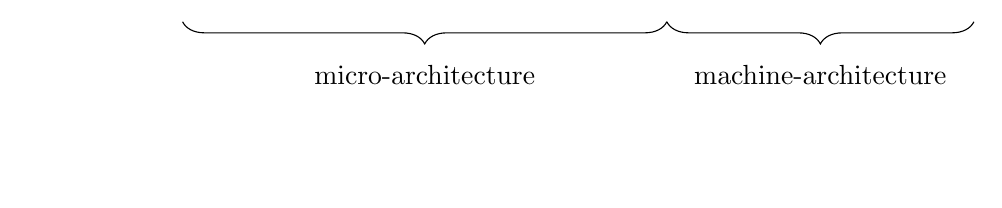
\begin{tikzpicture}
    \node at (0, 0) {}; % dummy node that placement works correctly
    \draw[transform canvas={yshift=1.1cm}, decorate,decoration={brace, amplitude=8pt, mirror, raise=6ex}] (1.85, 0) -- (8, 0) node[midway, yshift=-4.5em]{\text{micro-architecture}};
    \draw[transform canvas={yshift=1.1cm}, decorate,decoration={brace, amplitude=8pt, mirror, raise=6ex}] (8, 0) -- (11.9, 0) node[midway, yshift=-4.5em]{\text{machine-architecture}};
\end{tikzpicture}
\vspace{-1cm}
\end{definition}
Note that this calculated theoretical peak \gls{flops} only serves as a sensible upper bound. 
A real-world example will not be guaranteed or even likely to achieve the calculated theoretical peak performance. 
Nevertheless, if all researchers agree on one way to calculate the theoretical peak \gls{flops}, it can be used as a baseline, making results between different papers more easily comparable. 

As an example, we compute the theoretical peak \gls{flops} for double precision floating point types and a machine with dual-socket \gls{amd} EPYC 9274F \glspl{cpu}~\cite{amd_amd_2022}, which will also be used as a hardware platform in the later chapters. 
This \gls{cpu} has support for \gls{fma}3 and \gls{avx}-512. 
However, in Zen4 \gls{avx}-512 is implemented by \enquote{double-pumping} two $\SI{256}{\bit}$ registers. 
This means that the \gls{avx}-512 unit can compute one \gls{fma} instruction in two consecutive clock cycles, resulting in a count of $\frac{2}{2}$~\cite{amd_amd_2023}. 
Additionally, the EPYC 9274F \glspl{cpu} has an all-core frequency of $\SI{4.1}{\giga\hertz}$ and $\num{24}$ physical cores. 
Therefore, according to \autoref{def:peak_flops}, the theoretical peak \gls{flops} of the example machine's dual-socket \gls{cpu} are: $2 \cdot 8 \cdot 1 \cdot \SI{4.1}{\giga\hertz} \cdot 24 \cdot 2 = \SI{3148.8}{\giga\flops}$.

To get a more empirical upper bound and to verify if our theoretical peak \gls{flops} do indeed make sense, we can use one of the standard \gls{hpc} benchmarks like the \gls{hpl} benchmark~\cite{petitet_hpl_2018}. 
In the case of the EPYC 9274F \gls{cpu}, I used the \gls{amd} provided pre-built \gls{hpl} version~\cite{amd_pre-built_2025} and ran it with the default settings. 
As a result, the utility reported a performance of $\SI{2765.6}{\giga\flops}$, which is only $\SI{12}{\percent}$ worse than our theoretically calculated value. 
This shows us that our theoretical peak \gls{flops} are not too conservative and do not dramatically overestimate the possible real-world performance of our \gls{cpu}. 

If we are interested in the actually achieved performance in \gls{flops}, we have two options. 
First, we can use a tool that automatically provides us with the \gls{flops} values when we execute our code, like NVIDIA's nvprof~\cite{nvidia_corporation_cuda_2025}, \gls{amd}'s rocprofv3~\cite{amd_using_2024}, or likwid-perfctr~\cite{thomas_gruber_likwid_2023}. 
Alternatively, if no such tool is available or the current programming framework or hardware platform is not supported, we can calculate the necessary floating point operations by hand and divide it by the elapsed walltime. 
However, we must be careful when doing so. 
For example, if our target hardware supports \gls{fma} operations, we have to count code that looks like, e.g., \code{c[i] += a[i] * b[i]} as a single floating point operation. 
Additionally, counting the number of floating point instructions for non-trivial operations like floating point divisions, square roots, or exponential functions is difficult. 
Such operations can be translated into a single machine instruction with higher-than-normal latency or throughput, a fixed number of machine instructions, or even a variable number of machine instructions. 
In practice, these operations are often counted as a single instruction. 
To get a better estimate, we would have to examine the generated assembly code to count the number of floating-point instructions that are actually generated. 

\begin{listing}
    \begin{moderncode}{cpp}
#pragma omp parallel for
for (std::size_t i = 0; i < N; ++i) {
    a[i] = b[i] + q * c[i];
}
    \end{moderncode}
    \caption{%
    The standard vector TRIAD function from the STREAM benchmark suite~\cite{mccalpin_memory_1995}. 
    }
    \label{code:stream_triad}
\end{listing}

For example, let's look at the TRIAD function from the STREAM benchmark suite~\cite{mccalpin_memory_1995} shown in \autoref{code:stream_triad}. 
We can see two floating point operations, a multiplication and an addition; however, since our example \gls{amd} EPYC 9274F \gls{cpu} supports \gls{fma} operations, we have to count these operations as a single instruction. 
Therefore, the number of floating point operations in \autoref{code:stream_triad} is directly based on the number of loop iterations \code{N}. 
Running this code with \code{N=1e12} on our dual-socket \gls{amd} EPYC 9274F \gls{cpu} machine results in a runtime of $\SI{1.308}{\second}$, which means $\SI{11.47}{\giga\flop}$. 
The same code profiled with likwid-perfctr reports $\SI{0}{\giga\flop}$. 


\todo{Beispiel stream/triad CPU benchmark + likwid output $\rightarrow$ verifizieren, dass die Berechnung halbwegs sinnvoll ist!}

\todo{sinnvolles beispiel}